\chapter{\label{II_1}Application d'une segmentation temporelle automatique}

Au sein du chapitre suivant, nous proposerons la mise en place d’un processus de \gls{segtemp} automatisée. Notre proposition, considère moins la segmentation comme un prérequis technique que comme une tâche documentaire à part entière, directement articulée à l’indexation. Nos recherches ont montré que les études sur le sujet restent cantonnées aux expérimentations scientifiques et qu'elles n'ont pas été appliquées au domaine des humanités numériques. Nous établirons ainsi un état des lieux de ces expérimentations, afin de proposer la mise en place d'un tel processus dans un contexte de gestion de collections audiovisuelles patrimoniales.    




\section{\label{II_1_A}Traitement audiovisuel automatique}


%marquer davantage la vision par ordinateur classique et la vision par ordinateur fondée sur le deep learning, bcp utilisée dans l'analyse de l'audiovisuel

\subsection{État des lieux}

Les technologies appliquées à l'analyse de contenus vidéo et audio, comprenant la computer vision et la reconnaissance de discours automatique (ASR) sont globalement désignées sous le terme de \gls{AudiovisualProcessing} (AVP)\footcite{noord2021}.

Appliquées à un grand nombre de données, ces technologies permettent de passer du \textit{"close"} au \textit{"distant viewing"}, c’est-à-dire d’une vue des données rapprochée, réduite, à une vue d’ensemble. \footcite{noord2021} Les tâches de traitement automatique permettraient en effet de passer de l’analyse manuelle de certaines archives audiovisuelles, à une vue d'ensemble sur les données afin d'en extraire les tendances globales, modifiant ainsi notre rapport à ces documents. 

Les tâches d’analyse automatique pouvant être appliquées aux documents audiovisuels sont multiples, regroupant notamment le traitement du signal sonore (reconnaissance des locuteurs, transcription et classification audio) et l’analyse d’images (reconnaissance faciale, détection et classification d’objets, extraction de textes). Les chercheurs analysant les objets visuels s’orientent de plus en plus vers le contenu audiovisuel, puisque la détection du mouvement constitue un levier déterminant pour la mise en place d’autres tâches automatiques de reconnaissance \footcite{brostow2009}. 

Toutefois, l’accès au contenu actionné par le flux vidéo exige une structuration spécifique. Si la détection automatique des plans dans un flux vidéo est maîtrisée puisqu’elle n’engage que des changements visibles techniquement dans l’image, la détection sémantique de séquences reste inexploitée. Comme le souligne Samarth Bhargav, “pouvoir détecter de manière fiable les limites des scènes constituerait un exploit technique incroyable, qui ouvrirait d'énormes perspectives pour l'analyse sémantique et narrative des séquences vidéo et cinématographiques. [Traduction personnelle]" \footnote{\textit{"reliably being able to detect scene boundaries would be an incredible technical feat, which would create tremendous potential for semantic and narrative analysis of video and film material"} \cite{bhargav2019}}.

En effet, de nombreux projets sont dédiés à l’analyse automatique de corpus audiovisuels, toutefois, aucun projet n’est concrètement dédié à la \gls{segtemp} en différentes \gls{sequence} afin d'en indexer le contenu. L’Institut National Audiovisuel (\gls{ina}), est notamment pionnier dans la proposition de projets d’analyse automatique appliquée à l’audiovisuel. L’\gls{ina} a par exemple mis en place un outil de segmentation, \textit{InaSpeechSegmenter}, toutefois dédié à la segmentation du discours entre hommes et femmes, dans une optique statistique \footcite{zotero-item-787}. Cet algorithme de segmentation, appliqué au son, ne peut être pris comme exemple d’application pour notre étude, centrée sur l’analyse du sens de l’image en mouvement.  

Par ailleurs, le projet \textit{MeMad}, réunit un ensemble d’outils dédiés à l’analyse automatique de l’audiovisuel développés par l’Université d’Aalto, EURECOM, l’INA et l'Université d'Helsinki \footcite{zotero-item-790}. Parmi les outils développés, nous pouvons citer par exemple un outil de traduction du discours (\textit{Speech translation}), l’outil \textit{InaFaceGender}, un outil de reconnaissance faciale (\textit{Face recognition}), un outil permetttant d’identifier la langue parlée (\textit{Spoken language identification}) \footcite{zotero-item-790}. Ces projets restent centrés sur l’analyse du son et du texte inclut dans l’image et ne peuvent donc pas être pris en compte dans notre analyse. 
Au sein de cette sous section, nous tenterons ainsi d'évaluer les outils et méthodes disponibles et dédiés au traitement audiovisuels, afin de proposer un processus adéquat. 

%https://www.ai4media.eu/  

%Groupe de recherche et de réflexion et de développement d’outils pour l’analyse des médias par l’IA : pas de modules dédiés à la segmentation par séquence. Modules développés : reconnaissance d’objets, génération de résumés, segmentation sémantique. Mais modules bcp basés sur les mécanismes d’auto-attention pour ‘l'analyse vidéo. Documentation des projets non accessible. Un outil intéressant de détection de chnagement de plans mais documentation non accessible : 
%source: voir word 

\subsection{La \gls{Vision par ordinateur}}

\subsubsection{La \gls{Vision par ordinateur} classique}

L’application des technologies d’intelligence artificielle au domaine des images (images fixe ou vidéo) est désignée sous le terme de \textit{computer vision}, \gls{Vision par ordinateur} en français. Le terme définit un sous-domaine d’application de l’intelligence artificielle qui permet d’entraîner un système d’\gls{ia} à l’analyse des images fixes ou en mouvement \footcite{stryker2025}. 

La \gls{Vision par ordinateur} s’appuie largement sur des modèles d' \gls{Apprentissage machine} (\textit{machine learning}), qui désigne une branche de l'\gls{ia} regroupant les techniques, méthodes et processus nécessaires afin de rendre une machine ou un système informatique plus intelligent \footcite{zotero-item-584}. L'\gls{Apprentissage machine} permet d’entraîner des algorithmes capables d’apprendre à partir de données d’entraînement, afin de prédire ou de prendre des décisions sur de nouvelles données \footcite{zotero-item-702}. La \gls{Vision par ordinateur} classique s’appuie sur l’\gls{Apprentissage machine} précisément pour sa capacité à entraîner des systèmes à prédire. En effet, les corpus d’images fixes et d’images en mouvement sont des phénomènes complexes à appréhender pour des algorithmes, contrairement à des données statistiques et mathématiques. La nature de ces corpus les rend imprévisibles autant dans leur forme que dans leur contenu. Les algorithmes d’intelligence artificielle ne peuvent donc pas seulement réaliser une analyse prédictive de ce type de corpus, définie par des critères mathématiques \footcite{mahony2020}. 

Les corpus audiovisuels nécessitent une analyse prédictive, que les algorithmes sont entraînés à réaliser via des méthodes d'\gls{Apprentissage machine} \footcite{mahony2020}. De plus, la plupart de ces corpus sont d’une taille conséquente, forçant ainsi la mise en place d'algorithmes de prédiction, puisque l’entraînement machine ne peut être mis en place sur l’ensemble des données, seulement sur un échantillon donné. 

\subsubsection{\gls{Vision par ordinateur} fondée sur l'\gls{Apprentissage profond}}

Pour des tâches telles que la segmentation en différentes séquences, qui implique l’analyse du contenu de l’image, sont utilisés des modèles d’intelligence artificielle reposant sur des réseaux de neurones, et notamment des \gls{Réseaux de neurones profonds} \footcite{norindr2023}. Ces modèles relèvent également de la \gls{Vision par ordinateur}, mais fondée sur l'\gls{Apprentissage profond}, permettant notamment de gérer l'analyse de flux vidéo. La méthode de mise en place de ces \gls{Réseaux de neurones profonds} en plusieurs couches, est désignée sous le terme de \textit{deep learning}, \gls{Apprentissage profond}, une sous-catégorie de l'\gls{Apprentissage machine}. L'\gls{Apprentissage profond} est basé sur des réseaux de neurones artificiels inspirés du fonctionnement du cerveau humain. Les neurones sont en réalité des cellules de calcul organisées en différentes couches qui interagissent les unes avec les autres afin de s’adapter aux données reçues, et de prendre une décision quelconque. Davantage entrainé que programmé, un modèle fondé sur l’\gls{Apprentissage profond} permet d’exécuter des tâches automatisées, réduisant le besoin d'intervention humaine, et améliorant ainsi le rapport cout-efficacité \footcite{mahony2020}. Il suffirait de fournir au modèle quelques images annotées, dont le réseau de neurones repèrerait les caractéristiques à analyser sur de nouvelles données \footcite{mahony2020}. Par rapport aux techniques traditionnelles de \gls{Vision par ordinateur}, l'\gls{Apprentissage profond} permet d’obtenir une plus grande précision dans les tâches d'analyse audiovisuelle telles que la classification d'images, la segmentation, la détection d'objets \footcite{mahony2020}.

\subsection{\gls{Transformers} et \gls{cnn}}

Au sein des réseaux de neurones, le type de réseau spécifiquement employé dans le domaine de la \gls{Vision par ordinateur} pour la classification d’images et la reconnaissance d’objets, est celui des \gls{cnn}. Appliqués à des corpus d’images, les \gls{cnn} peuvent par exemple analyser une image selon une hiérarchie de caractéristiques afin d’en extraire les couleurs et les contours \footcite{brachmann2017}. Les tâches que permettent les \gls{cnn} sont plutôt bien adaptées à l’image fixe, puisqu’ils extraient des éléments fixes de l’image.  

Néanmoins, d’autres modèles issus de l'\gls{Apprentissage profond} tels que les \gls{Transformers} s’avèrent davantage efficace sur des tâches dédiées à l’image en mouvement, dont fait partie la segmentation. Contrairement aux \gls{cnn}, les \gls{Transformers} fonctionnent grâce à un mécanisme d’auto-attention qui leur permet de détecter les relations et dépendances entre les données \footcite{bergmann2025}. Tandis que les \gls{cnn} analysent les données de manière locale dans l'image, sans prendre en compte les interdépendances qui les régissent temporellement, les \gls{Transformers} examinent simultanément les données dans leur ensemble et décident de se concentrer sur certaines étapes de chacune d'entre elles \footcite{bergmann2025}. Les \gls{cnn} ne permettent pas, par exemple, de discerner les “dépendances à longue portée” telles que les corrélations entre les pixels entre différentes images qui ne seraient pas voisins \footcite{bergmann2025}. Ainsi, ils seraient davantage adaptés à l’analyse d’images en mouvement puisqu’ils prendraient en compte les relations entre les images, tandis que les \gls{cnn} seraient davantage adaptés aux images fixes.  Idéalement, la mise en place d’une segmentation automatique des archives audiovisuelles doit donc être fondée sur une architecture de type \gls{Transformers}.  


Toutefois, dans un contexte patrimonial, avec des ressources limitées, ces algorithmes fondés sur l’intelligence artificielle possèdent leurs limites. Premièrement, les réseaux de neurones sont conçus comme des boites noires, ne permettant pas d’interpréter les analyses qui sont produites \footcite{brachmann2017}. En effet, une fois entraînés, il est difficile d’en modifier les paramètres puisqu’ils sont entremêlés entre les différentes cellules de calcul. La réflexion produite est ainsi difficile à comprendre et à exposer\footcite{mahony2020}. 

Deuxièmement, les algorithmes de type \gls{Transformers} sont complexes et restent difficiles à adapter à un corpus audiovisuel lui-même complexe \footcite{yuan2025}. Ils demandent également de grandes puissances de calcul et un temps de paramétrage important, ce qui les rend inadaptés à des contextes de gestion de collections patrimoniales. De plus, ils requièrent un grand nombre de paramètres issu d’un large jeu de données d’entraînement afin d’éviter un surapprentissage impliquant des biais multiples \footcite{pattichis2023}. Ces modèles sont, de surcroit, généralement entraînés sur des jeux de donénes inadaptés, qu'il s'agirait de réadapter à un contexte patrimonial \footcite{pattichis2023}. Cette réadaptation impliquerait un temps conséquent dédié à la validation et à la correction de l'analyse automatique produite. Certaines approches algorithmiques non neuronales ou hybrides, qui combineraient \gls{Vision par ordinateur} et \gls{cnn} par exemple, seraient ainsi davantage adaptées car fondées sur des calculs et des seuils mathématiques les rendant plus stables. 
Ainsi, la nature de chaque modèle conditionne la qualité d'analyse automatique d'un flux vidéo. Afin de synthétiser les apports et les contraintes de ces différentes approches, le Tableau \ref{tab:comparatif_avp} ci-dessous permet de comparer les compétences des types de modèles cités pour l'analyse d'un flux vidéo. 


\begin{table}[H]
	\centering
	\small
	\renewcommand{\arraystretch}{1.3} %spécification de l'espace vertical
	\begin{tabular}{|p{3.6cm}|p{6.2cm}|p{6.2cm}|} %largeur des colonnes
		\hline
		\textbf{Type d'approche} & \textbf{Performances appliquées au flux vidéo} & \textbf{Limites} \\
		\hline
		\textbf{Vision par ordinateur classique} 
		& - Détection de changements de plan \newline
		- Calcul d'histogrammes et variations de couleurs \newline
		- Détection basique de mouvement par seuils
		& - Détection strictement syntaxique, sans extraction du sens \newline
		- Absence de reconnaissance d'objets ou de concepts \newline
		- Sensibilité à tous les types de mouvement, y compris les mouvements involontaires \\
		\hline
		\textbf{Apprentissage profond : CNN} 
		& - Classification d'images fixes extraites du flux vidéo \newline
		- Détection d'objets ou caractéristiques dans l'image
		& - Absence de compréhension des relations contextuelles entre les images \newline
		- Incapacité à saisir les dépendances spatio-temporelles \\
		\hline
		\textbf{Apprentissage profond : Transformers} 
		& - Segmentation sémantique et temporelle du flux \newline
		- Analyse du contexte narratif et des relations longues
		& - Nécessite des infrastructures lourdes à la puissance de calcul conéquente \newline
		- Nécessite un entraînement exigeant fondé sur des jeux de données volumineux et adaptés \\
		\hline
	\end{tabular}
	\caption{Comparatif des approches de traitement audiovisuel automatique}
	\label{tab:comparatif_avp}
\end{table}

Comme l'illustre le Tableau~\ref{tab:comparatif_avp}, si les architectures fondées sur les \gls{Transformers} offrent des compétences puissantes, notamment pour l'automatisation de la segmentation temporelle, ces architectures reposent toutefois sur de lourdes puissances de calcul ainsi que sur des jeux de données d'entraînement conséquents. À l'inverse, la \gls{Vision par ordinateur} classique offre une stabilité d'analyse de la syntaxe audiovisuelle, qui ne permet pas toutefois d'en extraire le sens. Ce constat justifie l'orientation de notre étude vers une approche hybride, combinant une architecture stable fondée sur la \gls{Vision par ordinateur} et sur des \gls{cnn} légers, afin de tenter de comprendre dans quelle mesure ces modèles peuvent segmenter un flux vidéo et en extraire des caractéristiques sémantiques.

% TODO: \usepackage{graphicx} required
%\begin{figure}
%	\centering
%	\includegraphics[width=0.7\linewidth]{images/screenshot001}
%	\caption{mahony2020}
%	\label{fig:screenshot001}
%\end{figure}


%transition vers la prochaine sous partie : parler des données d'entrainement (cf fichier IAvideo pattichis)

%Toutes les tâches automatiques qui peuvent être appliquées à la vidéo nécessitent un entraînement multimodal : 
%entrainement multimodal :  When we refer to multimodal or cross-modal learning, we are referring to learning using video, audio and/or text. These approaches generalize to a greater variety of visual tasks including action step localization, action segmentation, text-to-video retrieval, video captioning. \footcite{schiappa2023}

\section{\label{II_1_B} Outils de segmentation automatique}

Différents projets, extérieurs au domaine du patrimoine, tentent de mettre en place des algorithmes de segmentation vidéo. Bien que ces projets mettent en place l'analyse automatique de corpus vidéos moins spécifiques que ceux constitués d'\gls{Archivesaudiovisuelles}, leur architecture donne des pistes d'expérimentations afin de pouvoir implémenter un tel processus automatique au sein d'un logiciel de gestion des collections. En effet, face aux limites des méthodes d'\gls{Apprentissage profond}, nous tenterons de montrer dans quelle mesure la \gls{Vision par ordinateur} classique, fondée sur une architecture plus stable, peut s'appliquer à la tâche automatique que nous souhaitons implémenter, la segmentation d'un flux vidéo en différentes séquences. L'optique de cette étude est de fournir une proposition d'implémentation de fonctionnalités automatiques au sein d'un outil de gestion des collections d'un point de vue métier, en prenant en compte les besoins utilisateurs.

\subsection{Décomposer le mouvement}

Tout d'abord, afin de pouvoir implémenter des algorithmes plus légers que ceux des \gls{Transformers}, une des solutions envisagée consisterait à transformer un flux d'images en mouvement en la série d'images fixes qui le composent. Ce processus écarterait notamment le besoin d'analyser les relations entre les images par un mécanisme d'auto-attention prévu par les \gls{Transformers}. En effet, le médium cinématographique se caractérise par l'enchaînement d'une succession d'images fixes produisant l'illusion du mouvement. La transformation de ce flux à l'état d'images fixes par un outil technique permettrait de pouvoir gérer l'analyse sémantique de ces images par des processus légers prévus par la \gls{Vision par ordinateur} classique. Ces images fixes pourraient ensuite être regroupées en séquences après une analyse de leurs différences syntaxiques. Grâce à ce procédé, pourraient être appliqués les mêmes procédés d'analyse que ceux prévus pour l'image fixe, fondés sur la \gls{Vision par ordinateur} classique. 

Cette segmentation d'un flux audiovisuel fondé sur les différences de syntaxe entre les \gls{plan} serait la condition préalable d'une analyse sémantique, regroupant ces \gls{plan} fixes en des \gls{sequence} sémantiques. Dans un article sur la mise en place d'un processus de \gls{segtemp}, Yuelin Xin prône notamment le découpage syntaxique tel que nous l'avons défini comme étape préliminaire à l'analyse sémantique des images par des modèles d'intelligence artificielle \footcite{xin2023}. La segmentation syntaxique d'un flux audiovisuel en différents \gls{plan} fixes servirait alors de filtre permettant la classification sémantique de ces \gls{plan}. 

Ainsi, la segmentation automatique d'un document audiovisuel en \gls{sequence}s serait fondée sur l'analyse préalable des différences entre les \gls{plan} fixes qui la composent. Ainsi, si la syntaxe visuelle de deux \gls{plan} fixes est jugée suffisamment différente selon un seuil mathématique prédéfini, ces \gls{plan} appartiendront à des \gls{sequence} distinctes\footcite{xin2023}. Ces \gls{plan} sont en réalité retenus par l'algorithme comme des \gls{imgcle} contenues au sein de chaque \gls{sequence}, calculées comme l'image la plus représentative de la présence des éléments dans un flux donné \footcite{xin2023}. Ce principe, qualifié de sélection de données, permet d'alléger nettement la puissance de calcul et la structure des algorithmes \footcite{xin2023}. Ces \gls{imgcle} seraient ensuite analysées par un algorithme fondé sur des \gls{cnn}, afin d'y ajouter une analyse sémantique et de les regrouper en \gls{sequence}s. 

\subsection{PySceneDetect}

Ce processus est notamment appliqué par la bibliothèque python \gls{pyscene} qui permet la segmentation d'un flux vidéo à l'aide de différents paramètres définis en amont \footcite{zotero-item-706}. Les images extraites peuvent ensuite être regroupées de manière thématique, une fois l'analyse de leurs différences syntaxiques effectuée. Sans toutefois extraire la totalité des images fixes qui composent une \gls{sequence} audiovisuelle, \gls{pyscene} permet d'en extraire les \gls{imgcle}, c'est-à-dire les principaux différents \gls{plan}.

\gls{pyscene} est un outil en accès libre fondé sur des tâches de \gls{Vision par ordinateur} classique (non fondé sur un algorithme d'\gls{ia}), qui concrétise la mise en oeuvre de la comparaison syntaxique d'images fixes. L'outil s'appuie sur des détecteurs mathématiques afin d'analyser les différences structurelles entre les \gls{imgcle} tirées d'une vidéo \footcite{zotero-item-708}. Il s’agit ainsi d’un outil basé sur des seuils et mesures visuelles mathématiques paramétrables, et ne nécesite pas d'entraînement particulier, comme c'est le cas des outils de \gls{Vision par ordinateur} fondés sur l'\gls{Apprentissage profond}. \gls{pyscene} permet d'isoler des \gls{imgcle} de l'image animée, de les regrouper par similarité et de les dissocier selon leurs différences. 

\subsection{Fonctionnement}

\subsubsection{Paramétrages}
Trois méthodes de détection sont proposées par l’outil : une détection des fondus entrants et sortants (méthode \textit{treshold}, qui repère les niveaux de noir dans l’image, une détection de coupes rapides qui repère les changements de contenu entre images (méthode \textit{detect-content}), et une détection de coupes fondée sur la différence d’un plan avec les \gls{plan} adjacents (méthode \textit{detect-adaptative}) \footcite{zotero-item-708}. 
En théorie, \gls{pyscene} isole des \gls{plan} fixes, correspondant à des ruptures syntaxiques dans un flux d'images, et non des \gls{sequence}s, unités de sens narratives. Néanmoins, \gls{pyscene} permet de contourner cette limite grâce à la flexibilité de son paramétrage. 
En effet, l'élévation de la valeur du seuil de détection ou la fixation d'une durée minimale de \gls{sequence} (\textit{min-scene-len}), l'outil est moins sensibles aux variations minimales entre images et ne déclenche une rupture qu'en cas de déctection de changements visuels majeurs tels que l'éclairage, le décor, la composition, etc \footcite{zotero-item-708}. Par ce biais, la segmentation syntaxique proposée par \gls{pyscene} pourrait permettre de diviser un flux vidéo en différentes \gls{sequence}s, que la variation visuelle permettrait de regrouper de manière sémantique. Une fois le processus finalisé, l'outil génère des marqueurs temporels sur les images extraites et enregistre automatiquement \gls{imgcle} associée à chaque \gls{sequence} retenue. Le diagramme de flux \ref{fig:pyscenedetect_pipeline} ci-dessous illustre la manière dont l'outil pourrait être paramétré afin de segmenter le flux vidéo en \gls{sequence}s.

\begin{figure}[H]
	\centering
	\begin{tikzpicture}[node distance=1.5cm, auto, >=stealth,
		block/.style={rectangle, draw, fill=blue!5, text width=2.6cm, text centered, rounded corners, minimum height=1.2cm, font=\small},
		decision/.style={diamond, draw, fill=orange!10, text width=2cm, text centered, inner sep=0pt, font=\small},
		line/.style={draw, ->, thick}]
		
		\node [block] (video) {\textbf{Flux Vidéo Continu}\\};
		\node [block, right=1cm of video] (subss) {\textbf{Extraction de plans}\\};
		\node [block, right=1cm of subss] (diff) {\textbf{Calcul d'écart}};
		\node [decision, below=1cm of diff] (seuil) {\textbf{Écart supérieur au Seuil ?}};
		\node [block, left=1cm of seuil] (continue) {\textbf{Même séquence}\\};
		\node [block, right=1.2cm of seuil] (cut) {\textbf{Nouvelle séquence}\\};
		\node [block, below=0.8cm of cut] (imgcle) {\textbf{Sauvegarde d'images-clés et marqueurs temporels}};
		
		
		% Liens
		\path [line] (video) -- (subss);
		\path [line] (subss) -- (diff);
		\path [line] (diff) -- (seuil);
		\path [line] (seuil) -- node [above] {Non} (continue);
		\path [line] (seuil) -- node [above] {Oui} (cut);
		\path [line] (cut) -- (imgcle);
		
	\end{tikzpicture}
	\caption{Schéma du processus de détection de coupures par \gls{pyscene}}
	\label{fig:pyscenedetect_pipeline}
\end{figure}

Pour chaque changement détecté, une nouvelle \gls{sequence} est ainsi créée et une \gls{imgcle} est automatiquement enregistrée, associée au fichier vidéo d'origine. Nous proposerons la réutilisation de cette image au sein du processus suivant, dédié à l'analyse sémantique des séquences préalablement détectées, afin de ne pas surcharger les algorithmes. Ce système permettrait ainsi d’alléger le processus d’analyse sémantique, puisque les algorithmes reçoivent des images fixes au lieu de fichiers vidéos plus ou moins lourds. 

\subsubsection{Limites}

Toutefois, certaines mises en application de l'outil soulignent ses limites. Dans un article sur l'\gls{Apprentissage profond} comme outil d'analyse du cinéma des premiers temps, Samarth Bhargav explique par exemple que l'outil détecte beaucoup plus de coupures de \gls{plan}s que nécessaire au sein de ce type de corpus \footcite{bhargav2019}. Ce problème peut être lié à la qualité amoindrie de ce type d'archives, même après numérisation ou restauration \footcite{bhargav2019}. En effet, la qualité de l'image détermine nécessairement la performance de l'outil d'analyse utilisé et des résultats reçus \footcite{norindr2023}. De plus, Samarth Bhargav souligne la nécessité de connaître de manière précise les modalités de paramétrage de l'outil, afin de pouvoir l'adapter adéquatement à la nature du corpus analysé \footcite{bhargav2019}. Toutefois, un des avantages majeurs de l'outil \gls{pyscene} est sa disponibilité et la possibilité de le mettre en oeuvre facilement et gratuitement. De plus, c'est un outil fondé sur des tâches classiques de \gls{Vision par ordinateur} analytiques qui ne nécessitent pas d'entraînement particulier. Son paramétrage est également documenté et facilement modifiable, contrairement à ceux des réseaux de neurones. 

\section{\label{II_1_C}Mise en application}

\subsection{Spécificités du corpus traité}
Au sein du chapitre suivant, nous mettrons à l’épreuve l’adaptabilité de l’outil que nous avons décrit pour la segmentation des vidéos en \gls{sequence}s, au corpus d'\gls{Archivesaudiovisuelles} géré au sein du logiciel de Skinsoft. Ce corpus est composé d'archives issues des années 1910 à 1920 essentiellement documentaires, construit par des plans fixes, en noir et blanc et muets. Nous tenterons d’appliquer le processus de segmentation proposé par \gls{pyscene} ur un tel corpus, afin d’en comprendre les données qui pourraient être générées. Le corpus, utilisé ici comme cas d'étude, se caractérise notamment par son ancienneté, et donc par la dégradation de la pellicule sur laquelle l’image s’inscrit. L'outil pourrait ainsi rencontrer des difficultés lors de l’identification des coupures et des changements de plans, brouillés par la dégradation de l’image. Toutefois, la structure du contenu de ces archives facilite la tâche de l’outil, composé d’une succession de \gls{plan}s fixes, dont les coupures sont suffisamment marquées, en fait un corpus relativement bien adapté à ce type de tâche automatique, qui pourrait identifier les coupes plus facilement.  

Par ailleurs, \gls{pyscene}, nous l’avons vu, est un outil dédié à la détection de coupures et à la segmentation d’un flux vidéo en différents plans. Or, dans cette étude, nous cherchons à montrer comment segmenter un flux audiovisuel en différentes séquences, unités sémantiques autonomes. Dès lors, comment paramétrer un tel outil pour la détection d'éléments sémantiques plus larges tels que les \gls{sequence}s ?  

\subsubsection{Paramètres appliqués}

Une solution envisagée serait d'augmenter la valeur du seuil de coupures (treshold), pour que l'outil ne détecte plus les micro-coupures entre les images mais des coupes plus larges, à l'échelle de séquences \footcite{zotero-item-708}. L'outil enregistrerait alors un changement de séquence seulement lors d'une rupture significative de l’espace-temps à l'image. Ce paramétrage reste toutefois limité puisque plusieurs plans adjacents peuvent être radicalement différents d’un point de vue syntaxique, tout en appartenant bien à la même \gls{sequence}. Par exemple, une même \gls{sequence} peut contenir un gros plan et un plan d'ensemble, dont la composition visuelle est bien différente. Dans le cas du corpus d'\gls{Archivesaudiovisuelles} décrit, les plans restent larges et fixes, montrant l'ensemble du décor dans lequel ils s'inscrivent. Ainsi, le paramétrage du seuil pourrait être adéquatement réglé pour la détection de changements de décor, sur ce corpus donné, afin de segmenter le flux vidéo en différentes \gls{sequence}s.  

Par ailleurs, il est possible de régler l’outil sur une durée minimale de détection de coupures à l’aide du paramètre \textit{"min-scene-len"}, pour que le processus n’effectue de coupures qu’après un laps de temps défini \footcite{zotero-item-708}. La définition de ce paramètre nécessite une analyse statistique du corpus segmenté afin d’en définir la durée moyenne d'une séquence. Au sein du logiciel de gestion des collections prévu par Skinsoft, l’institution qui gère ce corpus d’archives documente déjà les séquences contenues par les différentes œuvres au sein des notices de films physiques, sous la forme de repères temporels. Une analyse statistique comparative pourrait être réalisée sur ces données documentées de \textit{time-codes} afin de déterminer la durée moyenne d'une séquence au sein du corpus. D'après nos observations, les séquences extraites sont généralement d'une durée de 60 secondes.

Enfin, sur ce corpus, le mode de détection adaptatif pourrait être privilégié, couplé à une analyse d'images plus importante, permettant à l’outil de comparer le contenu visuel d’un plan par rapport à une grande variété de plans qui l’entourent \footcite{zotero-item-708}. Ce paramètre permettrait encore de régler l’outil sur la détection de changements majeurs dans l'image, dans l'optique d'en extraire uniquement les \gls{sequence}s.  

\subsubsection{Données produites}
Une fois ces paramètres définis, le processus une fois enclenché produit deux types de données en sortie. D'une part, un fichier JSON ou CSV contenant les \textit{time-codes} de début et de fin correspondant aux séquences identifiées au sein de chaque fichier vidéo ingesté. Chaque \gls{sequence} est alors associée à un identifiant unique et à des \textit{times-codes} de début et de fin. D'autre part, l'outil permet également d'extraire pour chaque \gls{sequence} un fichier image, qui correspond à l'image fixe médiane, censée être la plus représentative de la séquence, désignée par le terme d'image clé \footcite{zotero-item-708}. 

Ainsi, la mise en application de l'outil \gls{pyscene}, de l'analyse des données d'origine jusqu'à la production des données de sortie, pourrait être schématisée de la manière suivante (\cref{figpyscene})


\begin{figure}[h!] 
	
	\centering 
	
	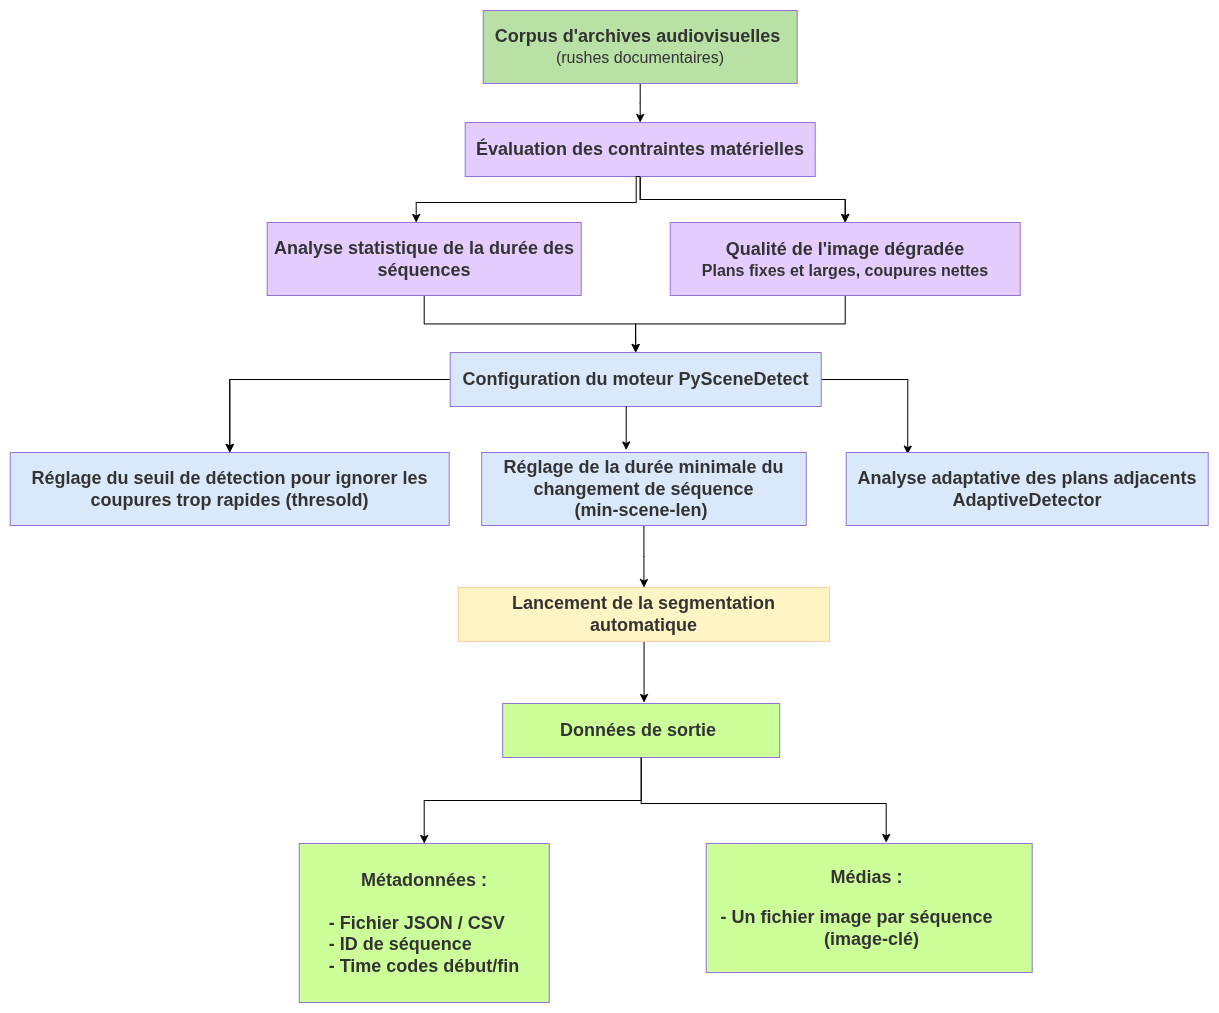
\includegraphics[width=1.0\textwidth]{images/pyscene.png} 
	
	\caption{Mise en application de \gls{pyscene}} 
	
	\label{figpyscene} 
	
\end{figure} 

Toutefois, si ce paramétrage permettrait une plus grande flexibilité pour la segmentation d’un flux vidéo en \gls{sequence}s, l’outil reste limité dans l’automatisation de cette tâche. D’une part l’outil est prévu pour la détection automatique de changement de plan, et d’autre part, une \gls{sequence} ne se définit pas seulement comme une caractéristique syntaxique du langage cinématographique, comme c'est le cas du plan, mais bien par une double caractéristique syntaxique et sémantique. En effet, un changement de séquence concrétise un choix narratif, matérialisé généralement par un changement d’espace-temps. C'est pourquoi, un outil dont l’automatisation est fondée sur des seuils mathématiques reste limité pour une telle tâche. Nous proposons alors de réaliser une analyse sémantique des \gls{sequence}s détectées, afin de ré-associer leur sens à ces coupures détectées automatiquement, tout en réutilisant les données produites : les \textit{times-codes} et l'image clé associés à chaque \gls{sequence}.  


Ainsi, la segmentation syntaxique effectuée par \gls{pyscene} constitue un “filtre”, c’est-à-dire un premier niveau dans notre chaîne d’indexation automatique des archives audiovisuelles \footcite{xin2023}. Les données issues de ce premier niveau permettent d’amoindrir le volume de données, caractéristique des fichiers vidéo, transmis aux algorithmes d’indexation automatique. Dès lors, les \gls{imgcle} produites par \gls{pyscene} peuvent être soumises à un modèle neuronal de détection d’objets tel que \gls{yolo} (\textit{You only look once}), afin d’extraire le sens de ces segments et leur rendre leur valeur sémantique. La sous-section suivante détaille la manière dont ce modèle, appliqué aux \gls{imgcle} issues des différentes \gls{sequence}, permet d’en extraire les caractéristiques sémantiques à des fins d’indexation.  




%Il est courant d’utiliser des modèles préentraînés sur un grand jeu de données et de le réajuster ensuite au jeu de données en question, au sein d’un contexte précis. \footcite{norindr2023} Ce modèle peut justement servir de modèle de caractéristiques à analyser sur les vidéos, un second entraînement, dans le contexte peut aider à l’affiner et à l’adapter au corpus spécifique. Le rendre d’abord familier au langage audiovisuel.  

%Malgré de grandes avancées dans le processing audiovisuel, avec des outils comme la computer vision appliquée à la vidéo, et la reconnaissance de discours automatique (ASR), ces outils restent largement inaccessibles et hors de portée pour les institutions patrimoniales. \footcite{noord2021}. Ils sont utilisés par des entreprises commerciales pour du montage vidéo par exemple. Le manque d'utilisation de ces outils dans le domaine des sciences humaines expliquent l'inexistance de données d'entraînement adaptées au secteur. \footcite{noord2021} 
%l'analyse vidéo par un processus humain prend un temps considérable, puiqu'il faut lire le fichier audiovisuel et en analyser les composants, le langage. Ainsi, l'indexation des archives audiovisuelles se cantonne souvent aux métadonnées, sans en exposer les données, le contenu.

%Et donc en pratique, comment appliquer le traitement audiovisuel à des corpus d'archives audiovisuelles patrimoniales ? 






%\subsubsection{entraîner ces outils et ces modèles}

%les modèles de détection neuronaux sont entrainés sur des datasets de clips courts. Or, la réalité auiovisuelle est bien différente. \footcite{pattichis2023} Des approches algorithmiques non neuronales ou hybrides seraient donc plus adaptées car fondée sur des calculs et des seuils matéhmatiques : plus stable. 

%détection des coupures : 
%approche algorithmique non neuronale (2SDS, pyscenedetect), (xin et attard) pipeline technique en 4 étapes (down sampling (miniaturisation), conversion en niveaux de gris, calcul d'empreinte numérique par hachage binaire des pixels, et calcul de la distance de Hamming pour marquer la rupture visuelle (xin2023)

%efficace sur les plans fixes et mvts lents 

%mettre en rapport avec les travaux d'Arnold  Tilton (2019), qui utilisent une méthode similaire combinant différences d'histogrammes et réduction de résolution des pixels (downsampling) pour mesurer les ruptures de palettes de couleurs et de luminosité d'une frame à l'autre, complétée par des règles logiques pour éviter les faux positifs lors des fondus (fade-in/fade-out).

%L'apport de l'IA (Vers la classification sémantique) : La détection brute des coupures ne suffit plus ; l'enjeu actuel est la Shot semantics (décrire le contenu d'un plan et sa typologie) (Arnold  Tilton, 2019).

%Le rôle des modèles (CNN et Détecteurs) : Pour analyser le contenu de ces plans, on utilise l'apprentissage supervisé (Supervised Learning), où des algorithmes apprennent à partir de données labellisées par l'humain (DeLua, 2024). C'est le cas des réseaux de neurones convolutifs (CNN) comme Faster R-CNN ou YOLO (un détecteur de type Single Shot qui prédit et classifie "en une seule fois") pour la détection d'objets ou de visages (Arnold  Tilton, 2019 ; Robert, 2026).

%Le méta-algorithme de classification : Arnold  Tilton (2019) montrent qu'en combinant la position des visages détectés et les coupures de plans, on peut créer un méta-algorithme capable de classifier automatiquement le type de plan (gros plan/close-up, plan amorce/over the shoulder), permettant de comprendre comment le cadrage construit le récit.

%\subsubsection{analyse du mouvement}

%au lieu d'utiliser des larges modèles qui tentent de tout classifier, plutot utiliser des modèles "low parameter", c'est-à-dire des modèles 3D-CNN légers, avec moins de paramètres dédiés à la reconnaissance d'une seule activité précise. prenennt moins de mémoire vidéo. \footcite{pattichis2023}

%stratégie de réduction de l'annotation humaine : slf supervised learning, semi supervised, active learning, zero shot \footcite{pattichis2023}

%confronter les architectures de réseaux de neurones (CNN vs. Transformers), introduire l'apprentissage non supervisé (Unsupervised Learning / DeepCluster),

%Les limites des CNN 2D classiques (comme ResNet) : ils analysent la vidéo comme des images discrètes et indépendantes, ignorant la continuité du mouvement \footcite{xin2023}. Se tourner vers les vision transformers : CLIP, ViViT (bergmann et al), mécanismes d'auto attention qui analysent l'intégralité d'une séquence

%Les modèles de Video Semantic Segmentation (VSS) et le dilemme entre les méthodes orientées "vitesse" (approche par keyframes peu précise) et orientées "précision" (TDNet, flux optique, mécanismes d'auto-attention) \footcite{zhou2022}.

%La gestion du coût de calcul : présentation de TDSNet (TFRM pour extraire les zones dynamiques par soustraction d'images consécutives, et MMRM pour pondérer selon la magnitude réelle du mouvement) \footcite{yuan2025}. règle ce dilemme 

%alternatives non supervisées : la supervision demande des données annotées (caron et al), l'apprentissage non supervisé (Unsupervised Learning) comme DeepCluster (Caron et al., 2018). Ce type de modèle regroupe les images ou frames similaires en "clusters" algorithmiques (via K-means) pour s'auto-entraîner sans intervention humaine (Caron et al., 2018). Si DeepCluster s'avère robuste face à des changements de distribution d'images (ce qui est prometteur pour des archives spécifiques), il présente deux limites majeures : il introduit des biais imprévisibles en remplaçant les labels par des métadonnées brutes (inacceptable pour la rigueur historienne) et a été conçu sur des bases gigantesques (ImageNet, 1.28 million d'images), le rendant difficilement transposable à des collections d'archives réduites (Caron et al., 2018 ; Norindr, 2023).

%infrastructure locale : amener l'algorithme aux données : C'est la discussion centrale de votre partie. Les outils d'AVP commerciaux (souvent basés sur le Cloud) sont inutilisables pour les archives en raison des droits de propriété intellectuelle et de la sécurité des données (van Noord et al., 2021). La solution réside dans des architectures locales comme DANE (projet CLARIAH), basées sur un système décentralisé de workers (van Noord et al., 2021). Ce type d'infrastructure produit des métadonnées exploitables, mais aussi des vecteurs de caractéristiques (représentations abstraites) ouvrant la voie à la recherche par similarité visuelle ou sonore (van Noord et al., 2021).

%La note finale sur l'explosion des données : L'indexation automatique par IA (comme avec DigInPix ou les modèles de type VLM) génère une masse d'informations locales phénoménale : les bases de données constituées peuvent être plus lourdes en taille que les fichiers vidéos d'origine (Moiraghi  Letessier, 2018).

%transition : nécessité d'un mapping vers le FRBR : faire correspondre la sortie de ces pipelines avec un modèle de données. 